\documentclass[a4paper,12pt]{report}
\usepackage[utf8x]{inputenc}
\usepackage[T1]{fontenc}
\usepackage[french]{babel} 
\usepackage{lmodern} % Pour changer le pack de police
\usepackage{makeidx}
\usepackage{graphicx}
\graphicspath{ {images/} }
\usepackage{wrapfig}
\usepackage{float}
\usepackage{verbatim}
\usepackage{moreverb}
\usepackage{listings}
\usepackage{float}

\setcounter{tocdepth}{3}     % Dans la table des matieres
\setcounter{secnumdepth}{3}  % Avec un numero.

\renewcommand \thesection       {\arabic{section}}
\renewcommand \thesubsection    {\thesection.\arabic{subsection}}
\renewcommand \thesubsubsection {\thesubsection.\arabic{subsubsection}}

\setlength{\parindent}{0cm}
\setlength{\parskip}{1ex plus 0.5ex minus 0.2ex}
\newcommand{\hsp}{\hspace{10pt}}
\newcommand{\HRule}{\rule{\linewidth}{0.5mm}}

\begin{document}

\renewcommand{\chaptername}{Partie}

\renewcommand{\contentsname}{Sommaire}

%###############
% PAGE DE GARDE 
%###############
\begin{titlepage}
  \begin{sffamily}
  \begin{center}

   ~% Upper part of the page. The '~' is needed because \\
   ~% only works if a paragraph has started.
    
\includegraphics[scale=0.1]{ufc.JPG}~~~~~~~
		
\includegraphics[scale=0.7]{ufr-st.jpg}\\[0.5cm]

    \textsc{\large Université de Franche-Comté}\\[0.2cm]

    \textsc{\large Master informatique - 1ère année}\\[1.25cm]
		
		\textsc{\huge Rapport de projet\\[0.2cm]Compilation et Génie Logiciel}\\[1.25cm]

   ~% Title
    \HRule\\
    { \huge \bfseries Interprétation et compilation en programmation objet\\ }

    \HRule \\[1.25cm]
    %\includegraphics[scale=0.5]{doc/chrono-env.png}
    %\\[1cm]

   ~% Author and supervisor
    \begin{minipage}{0.4\textwidth}
      \begin{flushleft} \large
				\emph{Auteurs~:}\\[0.5cm]
				Awa \textsc{Diallo}\\[0.2cm]
				Guzal \textsc{Khusanova}\\[0.2cm]
				Virgil \textsc{Manrique}\\[0.2cm]
				Mohammad \textsc{Nauval}\\[0.2cm]
				Jérémy \textsc{Navion}\\[0.2cm]
				Mehdi \textsc{Zemmoura}\\
      \end{flushleft}
    \end{minipage}\\[1.25cm]
		
		\textsc{\large Année universitaire 2017 - 2018}

  \end{center}
  \end{sffamily}
\end{titlepage}

%##########
% SOMMAIRE
%##########
\newpage
\tableofcontents

%###############
% REMERCIEMENTS
%###############
\chapter*{Remerciements}
\addcontentsline{toc}{chapter}{\protect\numberline{}Remerciements}
\paragraph{}
Au terme de ce travail, nous souhaitons remercier pour leur aide et leurs conseils xxxxxxxxxxxxx, [titres].

%##############
% INTRODUCTION
%##############
\chapter*{Introduction}
\addcontentsline{toc}{chapter}{\protect\numberline{}Introduction}
\paragraph{}
Dans le cadre de notre formation universitaire en première année de Master informatique, nous sommes amenés à réaliser un projet de compilation.
\paragraph{}
Contexte : pluridisciplinaire (COMP / GL) ; méthode agile par six ; rapport technique ; rapport GL séparé...
\paragraph{}
Les objectifs généraux de ce projet...
\paragraph{}
Nous débuterons par... Nous enchaînerons par..., et nous poursuivrons par... Pour terminer, nous ferons les bilans technique de ce projet.

%###############
% 1. LE PROJET
%###############
\chapter{Le projet de compilation}
%++++++++++++
% 1.1. SUJET
%++++++++++++
\section{Le sujet}
\paragraph{}
Objectifs détaillés...
%+++++++++++++++++++++++++
% 1.2. CAHIER DES CHARGES
%+++++++++++++++++++++++++
\section{Le cahier des charges}
\paragraph{}
Contraintes fonctionnelles / non fonctionnelles ; complète le sujet...
%++++++++++++++++++++++++++++++++
% 1.3. DECOMPOSITION / STRUCTURE
%++++++++++++++++++++++++++++++++
\section{Décomposition et architecture du logiciel}
\paragraph{}
Découpage en plusieurs parties : GUI, analyseur, compilateur, etc.

%############################
% 2. PARTIES / DEVELOPPEMENT
%############################
\chapter{Développement}
\paragraph{}
Nous étudierons d'abord... Nous expliquerons..., nous évoquerons ensuite..., nous poursuivrons par..., et nous terminerons par...
%++++++++++++++++++++++++++
% 2.1. CONTROLLEUR DE TYPE
%++++++++++++++++++++++++++
\section{Le contrôleur de type}
\paragraph{}

%+++++++++++++++++++++++++++++
% 2.2. ANALYSEUR
%+++++++++++++++++++++++++++++
\section{L'analyseur}
Cette partie est consacrée au module « Analyseur ». Elle contient des informations sur la grammaire, le parseur Minijaja et des utilitaires qui facilitent la gestion du langage qui vont être plus détaillés prochainement.
 
Premièrement, nous nous familiarisons avec des sous-parties (fichiers) intéressantes de l’analyseur et nous nous concentrons sur les principaux choix de réalisation. Ensuite, la discussion porte sur le traitement des erreurs (exceptions). Nous finissons par les tests réalisés.

\subsection{La grammaire et parseur MiniJaja}
Le fichier contient la grammaire MiniJaja décrit dans le langage JJTree . Ensuite, à partir du fichier MiniJajaGrammar.jjt, le parseur du Minijaja (MiniJajaGrammar.java), les nœuds d'arbres syntaxique abstraits (AST), et un visiteur de la grammaire sont générés à l’aide du compilateur javacc/jjtree.

Nous avons choisi d’utiliser les compilateurs javacc et jjtree qui permettent de générer le parseur à partir d'une grammaire donnée, car écrire notre propre parseur est plus complexe et plus couteux en temps. Ainsi, la grammaire donnée à l’entrée des compilateurs est sous forme BNF et en LL(1) (grammaire non-récursive à gauche et non-ambiguë). Pour rendre la grammaire MiniJaja proposée dans le support du cours de Compilation LL(1), nous avons utilisé les propriétés du langage Jjtree. 

Prenons comme exemple la déclaration d'une variable et d'une méthode :

decl$\,\to\,$var  |  methode

var$\,\to\,$typemeth ident vexp | typemeth ident [ exp ] |final type ident vexp

methode$\,\to\,$typemeth ident (entêtes) { vars instrs }

Il faut noter que "typemeth ident" rend la grammaire ambiguë. Pour résoudre ce problème,  nous avons mis le paramètre de jjtree lookhead à trois. Ainsi, avant prendre la décision pour le nœud déclaration, le parseur analyse d'abord les trois tokens suivants. Mais, nous avons décidé de transformer la grammaire en LL(1). Alors, ce est résolu à la manière suivante : 
 
\lstset{language=Java}
\begin{lstlisting}
void Declaration() #void: 
{}
{
  Constant()
| MethodType() Identifier() (Method() | Variable())

}
void Method() #void: 
{}
{
   <OPEN_PARENTHESIS> Parameters() <CLOSE_PARENTHESIS>
  <OPEN_CURLY_BRACKET> Variables() Instructions()  <CLOSE_CURLY_BRACKET> #Method(5)
}  
\end{lstlisting}

Remarques :
Les noeuds AST \#void ne sont pas générés.

Le noeud Method a cinq enfants, il va chercher les cinq derniers nœuds avant d'appeler \#Method(5)~: Instructions, Variables, Parametres, Identifier, MethodType.

\subsection{Visiteurs de la grammaire Minijaja }
La classe MiniJajaGrammarVisitor.java est un visiteur de l’arbre syntaxique de MiniJaja généré. Deux visiteurs qui héritent de ce visiteur ont été développés afin d'alléger le code de certaines implémentations du visiteur. Par exemple, la classe privée RevokeVisitor de la classe MiniJajaCompiler a surchargé quatre méthodes de DefaultMiniJajaGrammarVisitor. Pourtant, le visiteur de MiniJaja contient quarante-quatre méthodes à surcharger.     

\subsection{Traitement des erreurs}
\subsection{Jeu de test}
Pour tester les cas nominaux de la grammaire, nous avons écrit la classe de test MiniJajaGrammarTest. Pour cela, nous avons implémenté MiniJajaGrammarVisitor. Le test de grammaire est effectué de la manière suivante : 

1. Nous avons du code source MiniJaja syntaxiquement correct, cela veut dire que le parseur ne leve pas d'exception.

2. On parse le code source à l'aide de MiniJajaGrammar.java, et on obtient l'arbre syntaxique. 

3. Notre visiteur parcours chaque nœud de notre arbre et construit au fur à mesure un rendu. 

4. Pour déterminer si le test passe, nous vérifions que le code source MiniJaja donné à l'entrée du visiteur est identique au rendu du visiteur.  

%++++++++++++++++++++++
% 2.3. COMPILATEUR
%++++++++++++++++++++++
\section{Le compilateur}
Dans cette partie du rapport la discussion porte sur les modules  « JajaCode » et « Compiler ». Premier contient des classes nécessaires pour la construction d’un objet JajaCode et deuxième c’est un visiteur Minjaja, qui prend à l’entrée l’arbre MiniJaja et sort le Jajacode correspondant. 

\subsection{Conception et traitement des erreurs}
Pour la construction de JajaCode le pattern « builder » a été mis en place. JajaCodeBuilder est constructeur de JajaCode qui contient une liste des instructions de JajaCode. Le compiler les remplie au fur à mesure. Une fois les instructions de JajaCode sont construits, le methode build() généré l’objet JajaCode qui contient la séquence des instructions JajaCodede.
  
De plus, pour rendre les instructions de JajaCode compréhensible aux utilisateurs (au format chaîne de caractère) la classe JajaCodeRenderer mis en place . JajaCodeRenderer utilise le pattern visiteur et  hérite de l’interface JajaCodeInstructions. 

MiniJajaCompiler consiste de deux visiteurs. La classe MiniJajaCompiler et sa classe privée  RevokeVisitor. Le visiteur RevokeVisitor est dédié au  retrait de déclaration. 

MiniJajaCompiler supposé de recevoir à l’entré le code source correct de MiniJaja, cela veut dire que avant de passé par compiler l’analyseur effectue l’analyse lexicale et syntaxique et contrôleur de type vérifier le compatibilité des typages, l’adéquation des valeurs. Alors le MiniJajaCompiler ne gère pas des erreurs. 

\subsection{Tests}
La classe test MiniJajaCompilerTest teste la compilation du code source MiniJaja vers JajaCode. Pour cela les exemples de support de cours et des travaux dirigé sont utilisés.  On donne à l’entrée MiniJajaCompiler un code source MiniJaja et reçoit en sortie l’objet JajaCode.  Ensuite on convertit chaque instruction de JajaCode obtenu aux chaînes de caractères à l’aide JajaCodeRenderer. Alors on vérifier bien que compilation MiniJaja correspond bien à JajaCode que nous attend. 


%++++++++++++++++++++++
% 2.4. INTERPRETEUR MJ
%++++++++++++++++++++++
\section{L'interpréteur MiniJaja}
\paragraph{}


%+++++++++++++++
% 2.5. MEMOIRE
%+++++++++++++++
\section{La gestion de la mémoire}
Dans cette partie, nous allons examiner l'implémentation de l'état mémoire dans notre projet de compilation. La mémoire est l'un des éléments importants du projet et elle sert à gérer le stockage de tous les données déclarées dans un programme Minijaja. Ces données peuvent être des variables des différents types, des tableaux, et des déclarations des méthodes. 

\subsection{Conception}
L'état mémoire du projet est composé de trois éléments : le dictionnaire de données, le tas, et la pile. Nous allons regarder la conception de chacun de ces trois éléments.

\subsubsection{Le Dictionnaire de Données}
Comme son nom indique, le dictionnaire de données contient les données déclarées dans un programme Minijaja. Le dictionnaire de données est une table de hachage. Une table de hachage est une implémentation du tableau associatif, elle permet une association clé-valeur. 

On peut accéder à chaque valeur du tableau par sa clé. L'accès se fait par une fonction de hachage qui transforme une clé en une valeur de hachage (un nombre) indexant les éléments de la table, ces derniers sont appelés \textit{buckets} en anglais. Il nécessite de stocker dans les \textit{buckets} la paire clé-valeur et pas uniquement la valeur.

Le fait de générer une valeur de hachage à partir d'une clé peut engendrer un problème d'une collision, c'est-à-dire que deux clé différents, pourront se retrouver associées à la même valeur de hachage et donc au même \textit{bucket}. Pour résoudre ce problème, premièrement nous devons choisir une bonne fonction de hachage pour minimiser la collision. La fonction de hachage que nous avons choisi la fonction de hachage FNV1.

\begin{figure}[H]
\begin{center}
	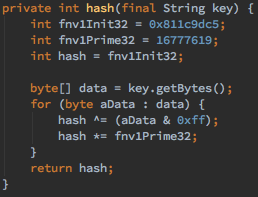
\includegraphics[scale=0.5]{hashfunction}
	\caption{Fonction de hachage FNV1}
\end{center}
\end{figure}

La fonction de hachage FNV1 n'est pas une fonction de hachage parfaite. Une fonction de hachage est dite parfaite si elle n'engendre aucune collision. En effet, nous avons toujours le problème de collision. Pour le résoudre, chaque case ou \textit{bucket} contient une liste chaînée. Si deux clés se retrouvent au même \textit{bucket}, les deux paires clé-valeur seront stockées dans cette liste.

Voici la représentation graphique de notre dictionnaire de données :
\begin{figure}[H]
\begin{center}
	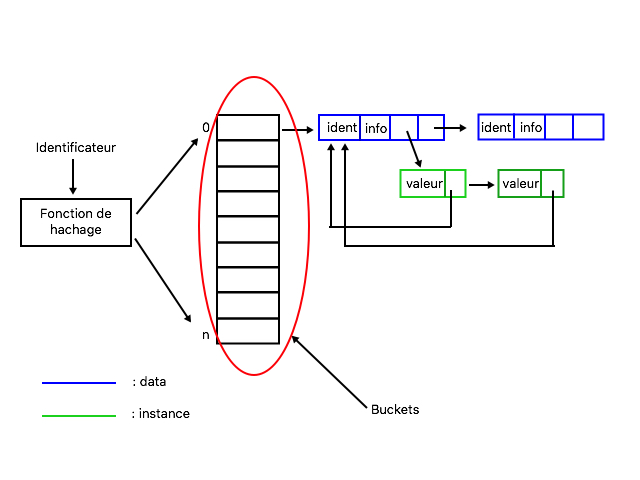
\includegraphics[scale=0.5]{hashmap}
	\caption{Dictionnaire de données}
\end{center}
\end{figure} 

L'image est notre dictionnaire de données. La table de hachage a pour capacité initiale \textbf{n}, c'est-à-dire qu'il contient n \textit{buckets}. Comme mentionné avant, chaque \textit{bucket} contient une liste de data. Data est un nœud de la liste, chaque data contient un identificateur, les informations concernant la variable, le tableau, ou la méthode déclarée. Chaque data possède une liste d'instances. Chaque instance possède une valeur et un pointeur vers son data pour récupérer les information concernant cette instance. 

Notre dictionnaire de données sert à stocker les données déclarées dans un programme Minijaja. Par exemple, lors du déclaration d'une variable de type entier:

\begin{lstlisting}
int test = 3;
\end{lstlisting}

Cette déclaration a pour l'identificateur la chaîne de caractères "test". Pour stocker cette déclaration dans le dictionnaire, on prends l'identificateur et on implémente la fonction de hachage à cet identificateur. Le résultat de cette fonction est un nombre qui indique l'indice du \textit{bucket} dans lequel la donnée sera stockée. Si, par exemple la fonction de hachage transforme la chaîne "test" en un nombre 0, on crée un nœud data, ce nœud a pour l'identificateur "test". La nature de l'objet est \textit{variable} et le type d'objet est \textit{integer}, ces deux informations sont aussi stockées dans le nœud data. Nous ajoutons aussi un nœud instance à la liste d'instances du nœud data, ce nœud instance a pour valeur 3. Nous ajoutons le nœud data à la liste chaînée du \textit{bucket} à l'indice 0.

Notre table de hachage a pour \textit{load factor} 0.75, c'est-à-dire que si le nombre d'éléments atteint 75\% de la capacité initiale, nous augmentons la capacité de la table de hachage. Ceci est fait pour diminuer la taille de la liste chaîne que chaque \textit{bucket} possède pour garder la complexité de la recherche d'un élément dans la table.

L'intérêt de l'utilisation de la table de hachage est la complexité de la recherche d'un élément. Comme les tables ordinaires, la table de hachage permet un accès en O(1) en moyenne. Toutefois, comme plusieurs paires clé-valeur peuvent se trouver dans un même \textit{bucket}, le temps d'accès dans le pire cas est de O(n).
 
 
\subsubsection{Le tas}
Le tas sert à stocker les données d'un tableau. Lors que l'utilisateur déclare un tableau d'une taille dans le programme Minijaja, les données de ce tableau sont stockées dans le tas. Le tas lui-même est un tableau.

Lors que le tas est initialisé, Le tas est initialisé avec une capacité donnée ou une capacité par défaut. Le capacité par défaut est de 256. Voici le tas après l'initialisation. Supposons que le tas a pour capacité sa capacité par défaut. Le tas possède un bloc libre de taille 256 à l'adresse 0.

\begin{figure}[H]
\begin{center}
	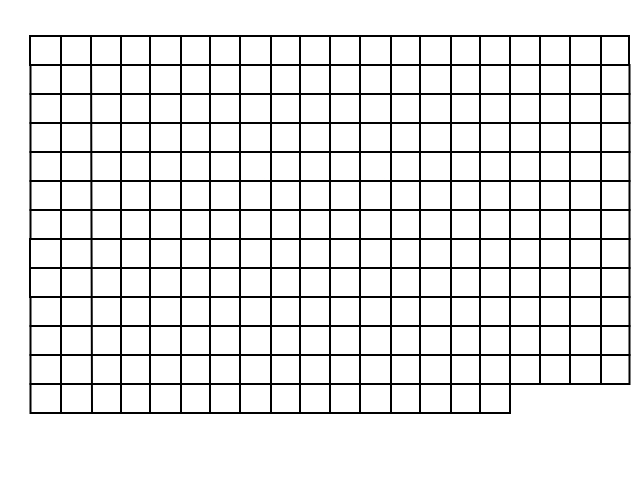
\includegraphics[scale=0.4]{initializetas}
	\caption{Initialisation du tas}
\end{center}
\end{figure} 

Nous avons aussi une table pour mémoriser les adresses des blocs libres dans le tes. Chaque case du tableau contient des adresses des blocs libres dont la taille est de 2 \^{} l'indice de la case dans le tableau. Par exemple, la case 0 contient des adresses des blocs libres de taille 2 \^{} 0 = 1.

Après l'initialisation du tas, la table d'adresses des blocs libres du tas indique qu'il y a un bloc libres de taille 256 à l'adresse 0.

\begin{figure}[H]
\begin{center}
	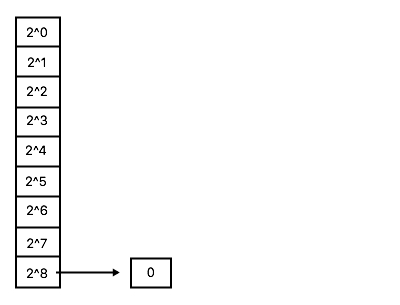
\includegraphics[scale=0.5]{adress}
	\caption{La table d'adresses des blocs libres du tas après l'initialisation du tas}
\end{center}
\end{figure}

Imaginons que l'utilisateur déclare un tableau "t1" de taille 10. Nous parcourons la table d'adresses pour chercher un bloc dont la taille est égale ou supérieure à 10. Nous avons trouvé un bloc de taille 256 à l'adresse 0. Ce bloc est ensuite découpé.

\begin{figure}[H]
\begin{center}
	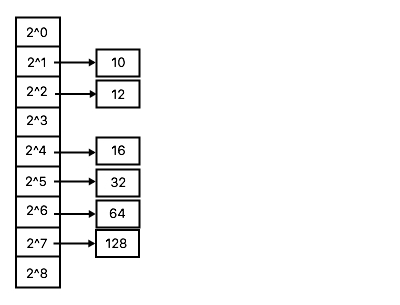
\includegraphics[scale=0.5]{adress2}
	\caption{Le tableau d'adresses des blocs libres du tas après la déclaration d'un tableau de taille 10}
\end{center}
\end{figure}

Nous pouvons regarder qu'il nous reste 6 blocs avec la taille totale de 246. Les éléments du tableau "t1" seront stocké dans le tas dans le bloc de taille 10 situé à l'adresse 0 jusqu'à l'adresse 9.

\begin{figure}[H]
\begin{center}
	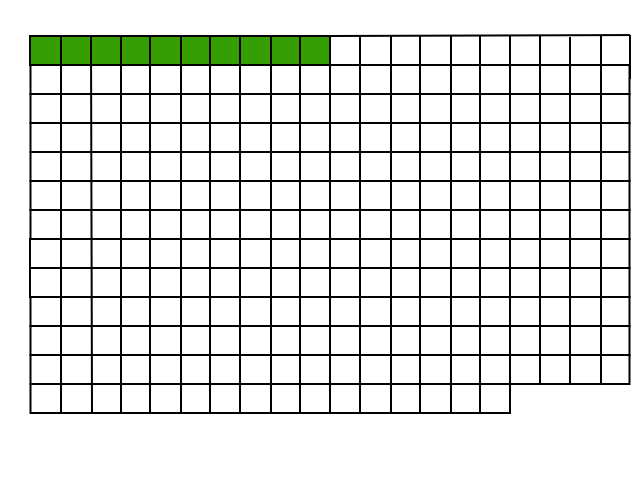
\includegraphics[scale=0.4]{tas2}
	\caption{Le tas après la déclaration du tableau de taille 10}
\end{center}
\end{figure}

Le bloc en vert est le bloc destiné à stocker les éléments du tableau "t1".

Supposons que l'utilisateur déclare ensuite un tableau "t2" de taille 3. Nous parcourons la table d'adresses de blocs libres, nous trouvons un bloc de taille 4 à l'adresse 12, nous découpons ce bloc.

\begin{figure}[H]
\begin{center}
	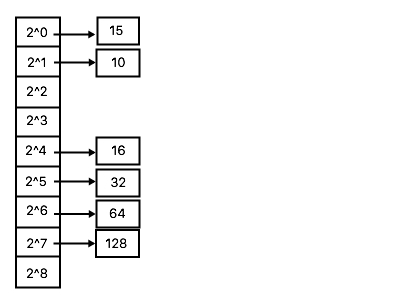
\includegraphics[scale=0.5]{adress3}
	\caption{La table d'adresses des blocs libres du tas après la déclaration d'un tableau de taille 3}
\end{center}
\end{figure}

En effet, les éléments du tableau "t2" seront stockés dans le bloc situé l'adresse 12 jusqu'à l'adresse 14.

\begin{figure}[H]
\begin{center}
	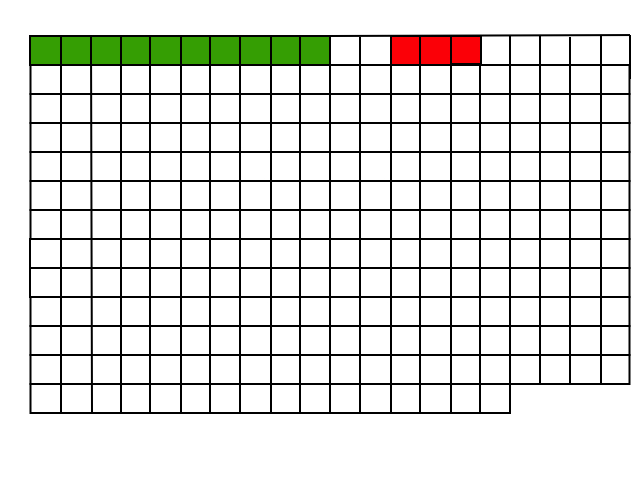
\includegraphics[scale=0.4]{tas3}
	\caption{Le tas après la déclaration du tableau de taille 3}
\end{center}
\end{figure}

Le bloc en rouge est le bloc destiné à stocker les éléments du tableau "t2".

Un problème apparaît. Comme ce que nous pouvons voir, il y a deux espaces libres entre le bloc en vert et le bloc en rouge, c'est le problème de fragmentation. Ces deux espaces risquent d'être perdu. Pour résoudre ce problème, nous faisons en sorte qu'à chaque déclaration du tableau, le bloc destiné à stocker ses données est aligné au plus gauche possible. Nous faisons aussi des fusionnement des blocs qui nécessitent d'être fusionnés.

\begin{figure}[H]
\begin{center}
	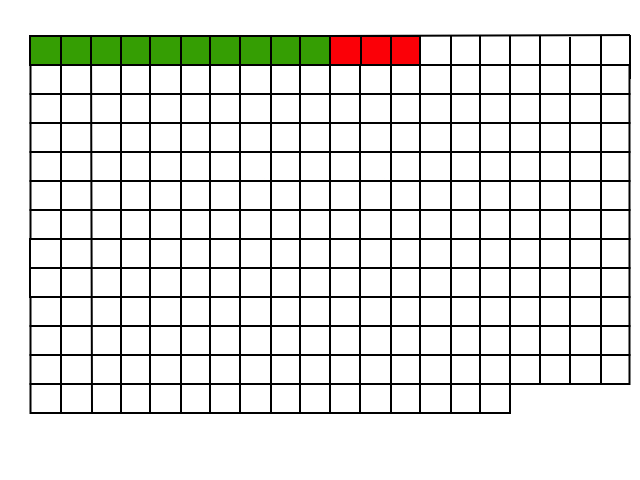
\includegraphics[scale=0.4]{tas4}
	\caption{Le nouveau bloc est aligné au plus gauche possible}
\end{center}
\end{figure}

\begin{figure}[H]
\begin{center}
	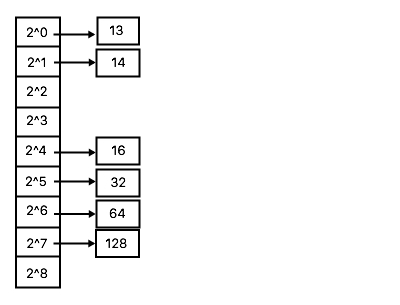
\includegraphics[scale=0.5]{adress4}
	\caption{La table d'adresses des blocs libres après l'alignement du bloc t2 au plus gauche possible}
\end{center}
\end{figure}

La même opération est faite lors de la suppression du bloc du tas. De cette manière, les blocs libres sont toujours regroupés à droite des blocs assignés. Et il n'y a pas de blocs libres situés entre des blocs assignés.

Nous avons aussi une table de symbole pour mémoriser les blocs assignés. Dans notre exemple, la table de symbole est comme ci-dessus:

\begin{figure}[H]
\begin{center}
	\begin{tabular}{ |c|c|c|c| }
	\hline
	Identificateur & adresse & taille & références \\
	\hline	
	1 & 0 & 10 & 1 \\
	\hline
	2 & 10 & 3 & 1 \\
	\hline
	\end{tabular}
	\caption{La table de symbole du tas}
\end{center}
\end{figure}

L'identificateur du bloc est la clé de cette table. Pour chaque clé, nous avons l'adresse du bloc, la taille du bloc, et aussi le nombre de références pour ce bloc. 


\subsubsection{La pile}
La pile sert à stocker les instances des variables, des tableaux, et des méthodes déclarées dans le programme Minijaja. Par exemple, lors de la déclaration des deux variables de type entier :

\begin{lstlisting}
int i = 3;
int j = 4;
\end{lstlisting}

Lors de la déclaration de ces deux variables, nous ajoutons à la table de hachage deux nœuds data, et nous ajoutons aussi deux instances à la pile. 

\begin{center}
	\textless i,INTEGER,VARIABLE,3\textgreater \\
	\textless j,INTEGER,VARIABLE,4\textgreater
\end{center}

Toutes les opérations se baseront sur la pile. Dans le cas où l'instance est un tableau, sa valeur est l'identificateur du bloc contenant les éléments du tableau dans le tas. Et dans le cas où l'instance est une méthode, sa valeur est le nœud AST de la méthode.

\subsubsection{La Mémoire}
La mémoire contient trois éléments : le dictionnaire de données, le tas, et la pile. Lors de la déclaration d'une donnée, l'identificateur et les informations de la donnée sont stocké dans le dictionnaire de données, la valeur de la donnée est stockée dans la pile. Dans le cas de la déclaration d'une tableau, ses éléments sont stockés dans le tas.

Les opérations qui peuvent être effectuées par la mémoire sont :

\begin{figure}[H]
\begin{center}
	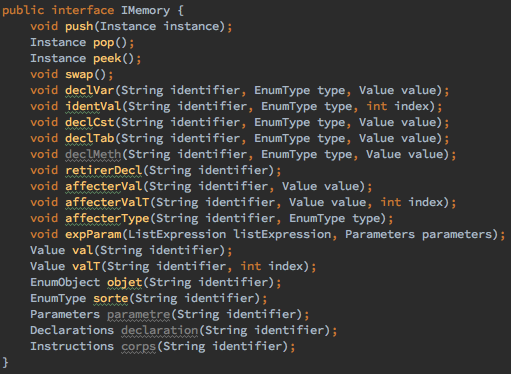
\includegraphics[scale=0.5]{memoire}
	\caption{Les opérations de la mémoire}
\end{center}
\end{figure}

\subsection{Traitement des erreurs}
Les erreurs peuvent apparaître lors des opérations dans la mémoire. Lors que une erreur est produite, une exception est levée. Par exemple, dans le cas où l'utilisateur essaie d'affecter une valeur à une variable dans la pile, mais la pile est vide. Une exception du type NullStackException est levée.

\begin{figure}[H]
\begin{center}
	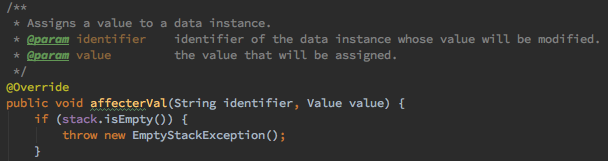
\includegraphics[scale=0.5]{affecterval}
	\caption{L'affectation de la variable dans le cas où la pile est vide}
\end{center}
\end{figure}

Il existe plusieurs autres exceptions dans la mémoire. Ces exceptions sont aussi utile pour le contrôle de type.

\subsection{Choix de tests}
Nous effectuons des tests fonctionnels pour chaque fonctionnalité de la mémoire et ses composants. Par exemple, la table de hachage est un composant de la mémoire, nous faisons des tests pour s'assurer que la table de hachage fonctionne correctement. Nous avons un test qui s'assure que la table de hachage augmente sa capacité si le nombre des éléments contenus dans la table de hachage atteint 75\% de sa capacité, nous avons aussi un test qui s'assure que lors de l'insertion d'une valeur avec une clé qui existe déjà dans la table de hachage, l'ancienne valeur est supprimée et remplacée par la nouvelle valeur. Voici la capture de ce test.

\begin{figure}[H]
\begin{center}
	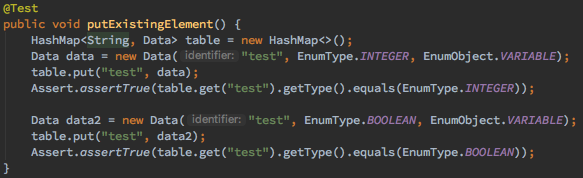
\includegraphics[scale=0.5]{testexisting}
	\caption{Un exemple du test fonctionnel de la table de hachage}
\end{center}
\end{figure}

Nous pouvons remarquer aussi que pour chaque test fonctionnel, nous déclarons de nouveau l'élément que nous testons. Dans l'image ci-dessus, nous déclarons la table de hachage au début du test. Nous n'utilisons pas une seule table de hachage pour tous les tests. Nous avons décidé de faire ce choix pour que chaque test ne dépend pas des autres test, autrement dit, chaque test est indépendant et peut être exécuté individuellement. 

Cependant, dans certains cas, nous avons besoin de tester une fonctionnalité avant de tester une autre fonctionnalité parce que la deuxième fonctionnalité a besoin d'appeler la première fonctionnalité. Par exemple, pour tester la méthode d'affectation d'une valeur à une variable dans la pile, nous avons besoin d'utiliser la méthode de la déclaration de la variable. C'est la raison pour laquelle nous devons être surs que la méthode de la déclaration de la variable fonctionne normalement avant de pouvoir l'utiliser. Autrement dit, nous avons besoin de tester la déclaration de la variable avant l'affectation de la valeur à une variable.

\begin{figure}[H]
\begin{center}
	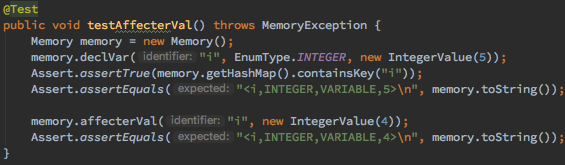
\includegraphics[scale=0.5]{testaffectation}
	\caption{Le test de l'affectation d'une valeur à une variable}
\end{center}
\end{figure}


%++++++++++++++++++++++
% 2.6. INTERPRETEUR JC
%++++++++++++++++++++++
\section{L'interpréteur JajaCode}
\paragraph{}
%++++++++++
% 2.7. GUI
%++++++++++
\section{L'Interface Homme-Machine}
\paragraph{}
Xxxx xxxxx....
%***********************************
% 2.7.1. Contraintes fonctionnelles
%***********************************
\subsection{Cahier des charges}
\paragraph{}
%******************************
% 2.7.2. Choix de réalisation
%******************************
\subsection{Choix de réalisation}
\paragraph{}
%********************
% 2.7.3. Conception
%********************
\subsection{Conception}
\paragraph{}
%***********************
% 2.7.4. Implémentation
%***********************
\subsection{Implémentation}
\paragraph{}
%**************
% 2.7.5. Tests
%**************
\subsection{Tests}
\paragraph{}
%******************
% 2.7.6. Résultats
%******************
\subsection{Bilan et résultats}
\paragraph{}

%##########
% 4. BILAN
%##########
\chapter{Bilan}
%+++++++++++
% 4.1. BILAN FONCTIONNEL
%+++++++++++
\section{Technique et Fonctionnel}
Tout d'abord, établissons le bilan technique et fonctionnel de notre projet. Commençons par les remarques importants sur le développement du projet. La première, au début du développement, la taille du projet nous a parue suffisamment conséquent et nous n'avons pas encore eu les connaissances techniques nécessaires pour comprendre le sujet du projet et commencer la phase du développement. 

Au fur et à mesure, nous avons pu comprendre le projet et son fonctionnement. Nous avons commencé petit à petit le développement. Tout au long de la période du développement, nous avons acquis des connaissances techniques qui nous ont permit à finir le projet.

Le support de cours proposé par M. Fabrice Bouquet nous a tellement aidé. Il nous a permit de pouvoir découper le projet en plusieurs module, comprendre les fonctionnalités de chaque module, et de comprendre ce qu'il fallait faire pour réaliser ces fonctionnalités.

Le support du cours nous a aussi permit de gagner du temps parce que nous avons pu utiliser les règles définies dans le support avec confiance. En plus, les travaux dirigés et les cours magistraux étaient très utiles dans la compréhension et l'avancement du projet.

Terminons par les difficultés que nous avons rencontrées. La première, c'était le fait que nous avons utilisé des techniques que nous n'avons pas encore acquis ou qui étions en cours d'être apprises. Cela nous a amené à négliger l'optimisation et la lisibilité des codes, sous condition qu'ils ont marché sans erreurs.

La deuxième, c'était le fait que c'était première expérience de l'utilisation des outils mis en place pour gérer la phase de \textit{build} du projet et faciliter la collaboration entre les membres de l'équipe (Maven, Jenkins, Nexus, SonarQube). Nous avons eu des difficultés à commercer l'utilisateur de outils mentionnés ci-dessus à cause de manque de l'expérience et parfois cela nous a freiné dans le développement. Cependant, nous avons eu la conscience que les outils utilisés sont utiles pour le développement de logiciel et c'était l'occasion de nous familiariser avec ces outils. En plus, la découverte de ces outils était assez intéressante pour nous. 

L'autre principale difficulté, c'était le fait que pour certains membres de l'équipe, les notions de tests n'étions pas encore complètement acquis. Cependant, c'était l'occasion de les apprendre.

%++++++++++++
% 4.2. BILAN PERSONNEL
%++++++++++++
\section{Personnel}
Sur le plan personnel, ce projet nous a apporté beaucoup de connaissances techniques pour chaque membre de l'équipe. La réalisation du projet a nécessité des efforts de chaque membre parce que sa taille est assez grande. 

Bien que le niveau technique de chaque membre de l'équipe diffère, nous avons pu avancer et réaliser le projet. Le fait que le projet est découpé en plusieurs module et chaque membre de l'équipe n'a pas travaillé sur tous les modules signifie que chaque membre n'a pas de compréhension des modules à lesquelles il n'a pas contribué.

%############
% CONCLUSION
%############
\chapter*{Conclusion}
\addcontentsline{toc}{chapter}{\protect\numberline{}Conclusion}

%#########
% ANNEXES
%#########
\appendix

%++++++++++
% ANNEXE A
%++++++++++
\chapter{Titre}

\newpage

%#########
% FIGURES
%#########
\listoffigures

%########
% RESUME
%########
\begin{abstract}
\paragraph{}
Dans le cadre...
\paragraph{}
As part of...
\paragraph{Mots clés}
Université de Franche-Comté...
\paragraph{Key words}
University of Franche-Comté...
\end{abstract}

\end{document}
